\documentclass{standalone}
\usepackage[ascii]{inputenc}
\usepackage{tikz}

\renewcommand{\familydefault}{\sfdefault}

\definecolor{TUMBlauHell}{RGB}{152,198,234} % Pantone 283

\begin{document}

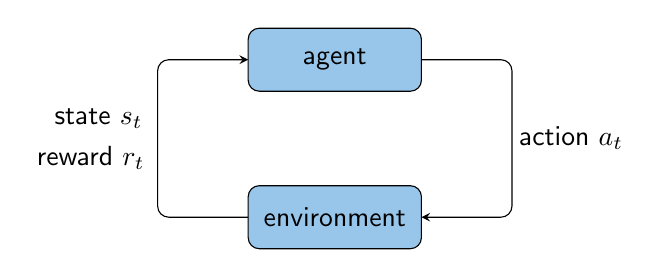
\begin{tikzpicture}[>=stealth]
\draw[rounded corners, fill=TUMBlauHell] (-1.1,  0.6) rectangle ( 1.1,  1.4);
\draw[rounded corners, fill=TUMBlauHell] (-1.1, -1.4) rectangle ( 1.1, -0.6);
\node at (0,  1) {agent};
\node at (0, -1) {environment};
\draw[->, rounded corners] ( 1.1,  1) -- ( 2.25, 1) -- ( 2.25,-1) -- ( 1.1, -1);
\draw[->, rounded corners] (-1.1, -1) -- (-2.25,-1) -- (-2.25, 1) -- (-1.1,  1);
\node at ( 3, 0) {action $a_t$};
\node at (-3,  0.25) {state $s_t$};
\node at (-3.1, -0.25) {reward $r_t$};
\end{tikzpicture}

\end{document}
